\documentclass[conference,onecolumn]{IEEEtran}

% =========================================================
% PLANTILLA LIGERA PARA OVERLEAF FREE
% Compilador recomendado: pdfLaTeX
% =========================================================

\usepackage[utf8]{inputenc}
\usepackage[T1]{fontenc}
\usepackage[spanish,es-nodecimaldot]{babel}
\usepackage{lmodern}
\usepackage{microtype}

\usepackage{amsmath,amssymb}
\usepackage{graphicx}
\usepackage{booktabs}
\usepackage{multirow}
\usepackage{array}
\usepackage{url}
\usepackage{cite}
\usepackage{xcolor}
\usepackage{listings}
% Se activan cuando el documento incluya algoritmos.
\usepackage{algorithm}
\usepackage{algpseudocode}
\usepackage{hyperref}

\definecolor{CodeBackground}{HTML}{F4F6F7}
\definecolor{CodeKeyword}{HTML}{005F73}
\definecolor{CodeComment}{HTML}{6C757D}
\definecolor{CodeString}{HTML}{BB3E03}

\hypersetup{
    colorlinks=true,
    linkcolor=black,
    citecolor=black,
    urlcolor=blue
}

\lstdefinestyle{paperstyle}{
    backgroundcolor=\color{CodeBackground},
    basicstyle=\ttfamily\footnotesize,
    keywordstyle=\color{CodeKeyword}\bfseries,
    commentstyle=\color{CodeComment}\itshape,
    stringstyle=\color{CodeString},
    numbers=left,
    numberstyle=\tiny,
    numbersep=5pt,
    frame=single,
    breaklines=true,
    showstringspaces=false,
    tabsize=4
}

\lstset{
    style=paperstyle,
    language=Python
}

% =========================================================
% DATOS DEL ARTÍCULO — EDITAR AQUÍ
% =========================================================

\title{
Parcial 2: Manejo y procesamiento de registros
}

\author{
\IEEEauthorblockN{
Kevin Javier Gonzalez Luna,
Iván Felipe Maluche Suarez,
Angélica Pascagaza Vega
}
\IEEEauthorblockA{
\textit{Universidad Nacional de Colombia}\\
\textit{Sede Bogotá}\\
Bogotá D.C., Colombia\\
\{kegonzalezl, imaluche, apascagaza\}@unal.edu.co
}
}
\begin{document}

\maketitle

% =========================================================
% RESUMEN
% =========================================================

\begin{abstract}
Este documento presenta los resultados de las implementaciones realizadas de heap y avl para el manejor de registros en el marco de posibles instrucciones que realizara un robot industrial
\end{abstract}

\begin{IEEEkeywords}
Arboles, BST, AVL, Max-Heap, Heap-sort, estructuras de datos
\end{IEEEkeywords}

% =========================================================
% CONTENIDO
% =========================================================
\section{problema elegido y diagrama de estructuras}
\subsection{enfoque elegido}
Se decidio implementar el sistema de registros para representar las tareas pendientes en un robot, consideramos que es un enofoque interesante para nosotros como ingenieros mecatronicos debido a la gran importancia de las ordenes secuenciales en la robotica industrial sumado a como este un campo de estudio es una de las principales areas de desarrollo de nuestra carrera y permite visualizar la integracion de las diferentes disciplinas que desarrolla la ingenieria mecatronica.

\subsection{diagrama basico de las estructuras de datos}
Para las implementaciones de las estructuras se decidio basar todas en una clase registro, a partir de esta dependiendo del caso se introducen directamente (heap) o por medio de un nodo.
\\
Hecho esto los ADTs implementados (heap, BST, AVL*, y arbol general) son usadas para la estructura del sistema de registros general el cual finalmente sera usado en el main.
\begin{figure}[h!]
    \centering
    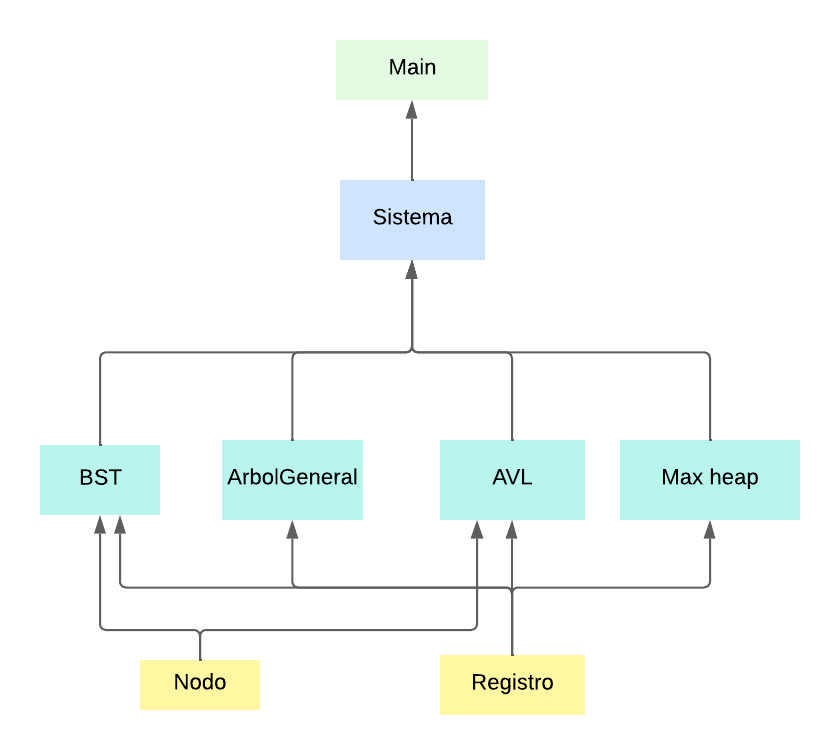
\includegraphics[width=0.5\textwidth]{imagenes/diagrama_general.png}
    \caption{Diagrama de estructuras de datos}
\end{figure}
\section{tabla de complejidades de las funciones implementadas}
\begin{table}[h!]
\centering
\caption{Tabla de Complejidades de Operaciones Estructurales}
\label{tab:complejidades}
\begin{tabular}{lll}
\toprule
\textbf{Operación} & \textbf{Mejor / promedio} & \textbf{Peor caso} \\
\midrule
Buscar en BST & $\theta(\log n)$ & $O(n)$ \\
Buscar en AVL & $\theta(\log n)$ & $O(\log n)$ \\
Insertar en AVL & $\theta(\log n)$ & $O(\log n)$ \\
\addlinespace % Espaciado para separar por categorías como en la imagen
Eliminar en AVL & $\theta(\log n)$ & $O(\log n)$ \\
Insertar en heap & $\theta(1)$ promedio & $O(\log n)$ \\
Extraer máximo del heap & $\theta(\log n)$ & $O(\log n)$ \\
Construir heap (\texttt{buildHeap}) & $\theta(n)$ & $O(n)$ \\
Heap-Sort & $\theta(n \log n)$ & $O(n \log n)$ \\
\addlinespace
Árbol general: buscar / cancelarSubarbol & $\theta(n)$ & $O(n)$ \\
CANCELAR (completo) & $\theta(n)$ & $O(n)$ \\
REPORTE & $\theta(k \log k)$ & $O(k \log k)$ \\
\bottomrule
\end{tabular}
\end{table}
\subsection{complejidad BST}
Para la busqueda siempre que el arbol este organizado se tendra complejidad logaritmica, pero en un caso donde el arbol degenere a una cadena esto se pierde (peor caso)
\subsection{complejidad AVL}
El problema anteriormente descrito con el AVL se arregla gracias a las rotaciones, gracias a esta misma la rotacion se mantiene en logaritmica al recorrer un camino de altura log(n), la eliminacion es un caso similar.
\subsection{complejidad Heap}
La insercion en un heap se basa en intercambios de nodos en funcion de la prioridad (o el ID en caso de empate), para la mejor situacion solo se comparara y se parara si se cumple la condicion del heap mientras que en el peor se tendra que subir por un camino de tamaño log(n) (pues el heap es aproximadamente balanceado si lo representamos como arbol)
\\
Para la extraccion el costo es similar pues hecha la extraccion (O(1)) se realizan intercambios de nodos desde el root por un camino log(n) aproximadamente
\\
Build heap a pesar de usar log(n) debido a los siftdown se realizara en un valor fijo de n veces por como recorre el arreglo original, dando por esto su magnitud lineal.
\\
Heap-sort despues de realizar un build heap (O(n)) realizar n veces un siftdown (O(log n)), comparando la magnitud que marca la tendencia de crecimiento es la de los n siftdowns (nlogn).
\subsection{complejidad del arbol general}
La busqueda busca en todos los nodos del arbol hasta encontrar el que encaje con la ID, se mantendra en magnitud lineal.
\\
Para la cancelacion del subarbol primero lo busca y entonces lo elimina, dando nuevamente una longitud lineal
\subsection{complejidad del sistema}
El Reporte realizar un heap sort (nlogn) y un bucle for de n elementos para representar el reporte (n), la magnitud que marca el crecimiento es O(nlogn)
\\
Cancelar ejecuta una busqueda de la id dentro del avl (log(n)), una cancelacion de subarbol dentro del arbol general (n) y una reconstruccion en el max-heap (n), comparando magnitudes la tendencia de crecimiento que lidera es lineal

\section{comparacion AVL y Heap}
Un BST y un AVL tienen grandes diferencias en eficiencia porque, aunque comparten la misma lógica de ordenamiento (todo hijo izquierdo es menor a su padre y todo hijo derecho es mayor a su padre), solo el AVL impone una condición de equilibrio que garantiza que la altura crezca de forma logarítmica.
En el caso de insertar claves ordenadas perjudica al BST porque este no aplica ningún rebalanceo, es decir, cada nueva clave mayor (o menor) que todas las anteriores desciende siempre por la misma rama, degenerando el árbol en una estructura lineal equivalente a una lista enlazada, con altura O(n) y búsquedas e inserciones en O(n). En contraste, el AVL verifica el factor de equilibrio de los nodos en cada inserción y aplica rotaciones ismples o dobles cuando la diferencia de alturas supera 1, lo que hace que la altura se mantiene acotada en O(log n) incluso con entradas ordenadas.
Al comparar las alturas, con las claves 1..7 el BST construido insertando en orden creciente resulta totalmente sesgado a la derecha: su altura es 6, pues cada clave se convierte en hijo derecho de la anterior. El AVL con esas mismas claves se equilibra mediante rotaciones y alcanza altura 2, la mínima posible para 7 nodos, ya que $2^3 - 1 = 7$. Con 1..1000 la diferencia es aún más marcada: el BST ordenado tiene altura 999 (lineal), mientras que el AVL mantiene altura cercana a $\log(1001) \approx 10$, es decir, un orden logarítmico.
\section{errores encontrados y decisiones tomadas en la implementacion}
\subsection{decisiones de implementacion relevantes}
\begin{itemize}
 \item Se decidio separar completamente la implementacion de arbol general de la de BST y de igual modo la de AVL de la de BST, esto se realizo por la dificultad para el grupo de realizar herencia entre clases, a pesar de ser algo posible de aprender consideramos que la diferencia no es significativa para el momento en el que habiamos caido en cuenta de esto.
 \item Se decidio implementar el registro como una misma clase usada en todas las estructuras para unificar el diseño del algoritmo entre todas las estructuras.
 \item Dentro de heap no se implemento directamente un arreglo dinamico debido a que no era estrictamente necesario, pues en la propia implementacion tomada como ejemplo se podia mantener las convenciones de indices del arreglo normal con tan solo poner un caso para el duplicado en vez de usar una clase completa con metodos no tan favorables para el flujo de programacion
\end{itemize}
\subsection{errores encontrados}
\begin{itemize}
 \item Inicialmente el siftdown y siftup del heap debido a la implementacion ineficiente de las condiciones del desempate no funcionaban correctamente, para solucionar esto se creo una funcion especifica para matener el condicional que mantenia los bucles en el heap original
 \item Para el arbol general se hizo uso de una clase nodo general, pues inicialmente se pensaba trabajar con el mismo nodo usado en BST mas la complejidad de mantenerlo para ambos caso orillo a crear uno propio para cada uno.
 \item Debido a la falta de conocimiento en java sin querer se asignaron nuevos punteros en algunos puntos del heap en vez de crear nuevos objetos, esto se soluciono con los comandos adecuados.
\end{itemize}
% =========================================================
% AGRADECIMIENTOS
% =========================================================
%ESTO ENTRA PARA POSTERIORES ENTREGAS
%\section*{Agradecimientos}

%Los autores agradecen a la Universidad Nacional de Colombia, Sede Amazonia,
%y a las personas o instituciones que apoyaron el desarrollo de este proyecto.

% =========================================================
% REFERENCIAS
% Sin BibTeX ni Biber para reducir tiempo de compilación.
% =========================================================



\end{document}
